%
% HSR LaTex Template
% Copyright 2012, Florian Bentele
%
% Additions by BA Team:
%  - Manuel Alabor
%  - Alexandre Joly
%  - Michael Weibel
%
% Complete LaTex template for thesis at HSR, customized
% for Prof. Dr. Peter Heinzmann
%
%
% This document is free software: you can redistribute
% it and/or modify it under the terms of the GNU
% General Public License as published by the Free
% Software Foundation, either version 3 of the License,
% or (at your option) any later version.
%
% This document is distributed in the hope that it will
% be useful, but WITHOUT ANY WARRANTY; without even the
% implied warranty of MERCHANTABILITY or FITNESS FOR A
% PARTICULAR PURPOSE. See the GNU General Public
% License for more details.
%
% You should have received a copy of the GNU General
% Public License along with this document. If not, see
% <http://www.gnu.org/licenses/>.
%

\documentclass{hsrthesis}

\makeindex

% do this here, so you can \gls{...} to it
%add new glossaryentries here...

\newglossaryentry{sqlite}{
	name=SQLite,
	description={SQLite ist eine Datenbankengine, welche ohne Konfiguration auskommt. Es handelt sich dabei um eine Datenbank in einer Datei},
	first={SQLite}
}
\makeglossaries

\begin{document}

%\begin{titlepage}
\title{Advanced Patterns and Frameworks}
\author{Manuel Alabor}
\date{FS 2013}
\maketitle
\end{titlepage}

\tableofcontents

\newpage

% The main content
%%%%%%%%%%%%%%%%%%
\chapter{Access Control Models}
\section{Authorization}

Das Authorization Pattern beschreibt auf einfache Art und Weise die Zugriffsberechtigungen eines Subjekts auf ein bestimmtes Objekt. Es spezifiziert zudem die Art des erlaubten Zugriffes (Lesend, schreibend etc.)

\subsection*{Kontext}
Jegliche Umgebungen in denen der Zugriff auf enthaltene Objekte kontrolliert werden muss.

\subsection*{Problem}
In einer kontrollierten Umgebung muss sichergestellt werden, dass nur berechtigte Subjekte auf entsprechende Objekte zugreifen können. Es stellt sich also die Herausforderung, diese Information losgelöst von den eigentlichen Objekte abzulegen. Dabei soll aber eine gewisse Flexibilität bei der Definition von Berechtigungen, Objekten und Subjekten erhalten bleiben.

Desweiteren sollen diese Informationen so einfach wie möglich im nachhinein änderbar sein.

\subsection*{Lösung}
Strukturell fällt die Lösung zum Authorization Pattern relativ simpel aus:

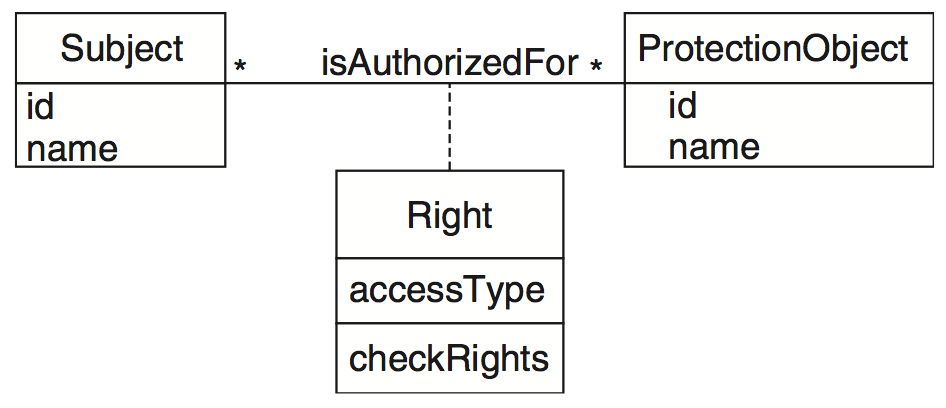
\includegraphics[width=50mm]{chapter/01basic/authorization.png}

\begin{itemize}
	\item Subject beschreibt jegliche Aspekte des zu berechtigendn Subjekts
	\item Das ProtectionObject ist das zu schützende Objekte
	\item Right enthält alle Informationen, wie Subject auf ProtectioObject zugriefen darf/kann
\end{itemize}

\subsection*{Erweiterungen}
Die vorgestellte Struktur kann um komplexere Aspekte erweitert werden. So kann bspw. mittels einem ''Copy''-Flag eine Stellvertretung eines Subjektes durch ein anderes ermöglicht werden.
Weiter ist die Verwendung eines Prädikats denkbar, welches eine Regel mit zusätzlicher ''Intelligenz'' austatten kann (-> ''Darf nur zugreifen wenn Zeit innerhalb Arbeitszeit'')

Diese Anpassungen können direkt auf dem Rights-Objekt modelliert werden.

\subsection*{Vor- \& Nachteile}
\begin{itemize}
	\item Durch seine Offen- und Allgemeinheit kann dieses Pattern auf jegliche Umgebung appliziert werden (Filesysteme, Organistaitonsstrukturen, Zugangskontrollen etc.)
	\item In der beschriebenen Form sind administrative Aufgaben (Änderung der Zugriffsrechte) nicht gesondert definiert. Für bessere Sicherheit ist dies jedoch von Vorteil
	\item Für viele Subjekte/Objekte müssen entsprechend viele Berechtigungsregeln erfasst und auch verwaltet werden
	\item Viele Regeln machen die Verwaltung für einen Administrator zu einer heikeln Aufgabe (Verkettung von Berechtigungen etc.)
\end{itemize}

\subsection*{Beispielanwendungen}
\begin{itemize}
	\item Dateisysteme
	\item Firewalls greifen teilweise auf dieses Pattern zurück, um Regeln für den analysierten Traffic zu modellieren
\end{itemize}
\section{Role Based Access Control}

Diese Pattern basiert stark auf dem Authorization Pattern und versucht dessen Nachteile durch einen zusätzlichen Abstraktionslayer auszugleichen.
Das ''Role Based Access Control'' Pattern definiert Berechtigungen nicht direkt auf Stufe der Subjekte, sondern versucht diese in Gruppen (Aufgabenbereiche, Kaderposition, Arbeitsort etc.) einzuteilen und anschliessend auf dieser Ebene quasi übergeordnet zu berechtigen.

\subsection*{Kontext}
Eine Umgebung mit vielen Objekten und Subjekten. Deren Berechtigungen ändern häufig. Zudem ist damit zu rechnen dass eben so oft neue Subjekte und Objekte hinzukommen oder wieder wegfallen.

\subsection*{Problem}
Die Rechteverwaltung in dem beschriebenen Kontext generiert einen hohen administrativen Aufwand. Um die Anzahl individueller Berechtigungen zu minimieren soll versucht werden, alle Subjekte in Gruppen einzuteilen. Die Einteilung basiert darauf, dass Subjekte mit ähnlichen Aufgaben zumeist auch ähnliche oder identische Berechtigungen benötigen.
Trotzdem sollen die Berechtigungen weiterhin präzise abgebildet werden können (''Need to know'').

\subsection*{Lösung}
Organisationen bieten normalerweise bereits mehr oder weniger wohldefinierte Gruppenstrukturen (Abteilungen, Aufgabenbereiche).
Ein gutes Sicherheitskonzept sollte bestrebt sein, dass jedes Subjekt genau auf die Objekte Zugriff hat, mit welchen es täglich arbeitet (wiederum ''Need to know'').

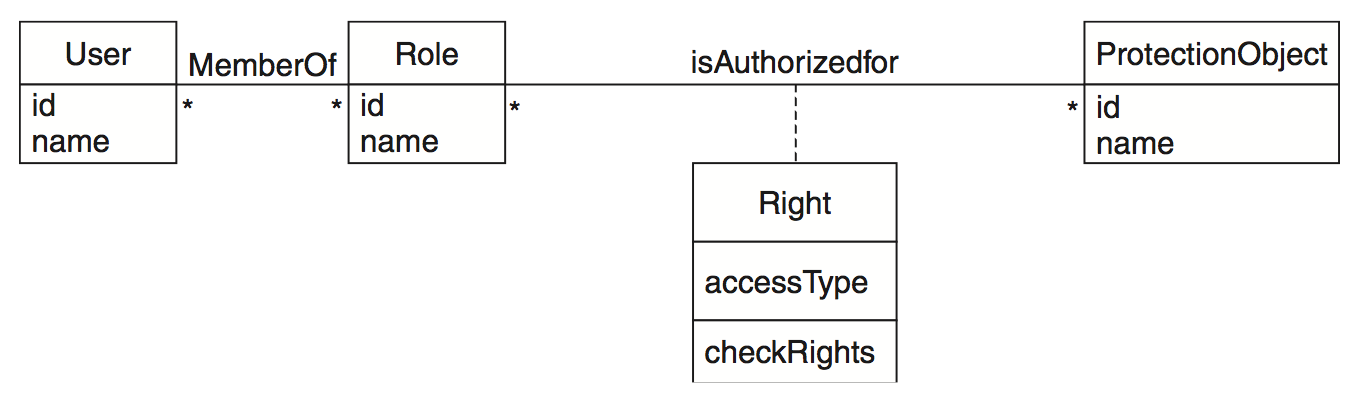
\includegraphics[width=\textwidth]{chapter/01basic/rolebasedaccesscontrol.png}

Im Vergleich zum Authorization Pattern kommt lediglich ein neues Element hinzu: Die Role fasst mehrere User (Subjekte) zu einer Menge zusammen und berechtigt sie über Right für ein spezifisches ProtectionObject.


\subsection*{Erweiterungen}
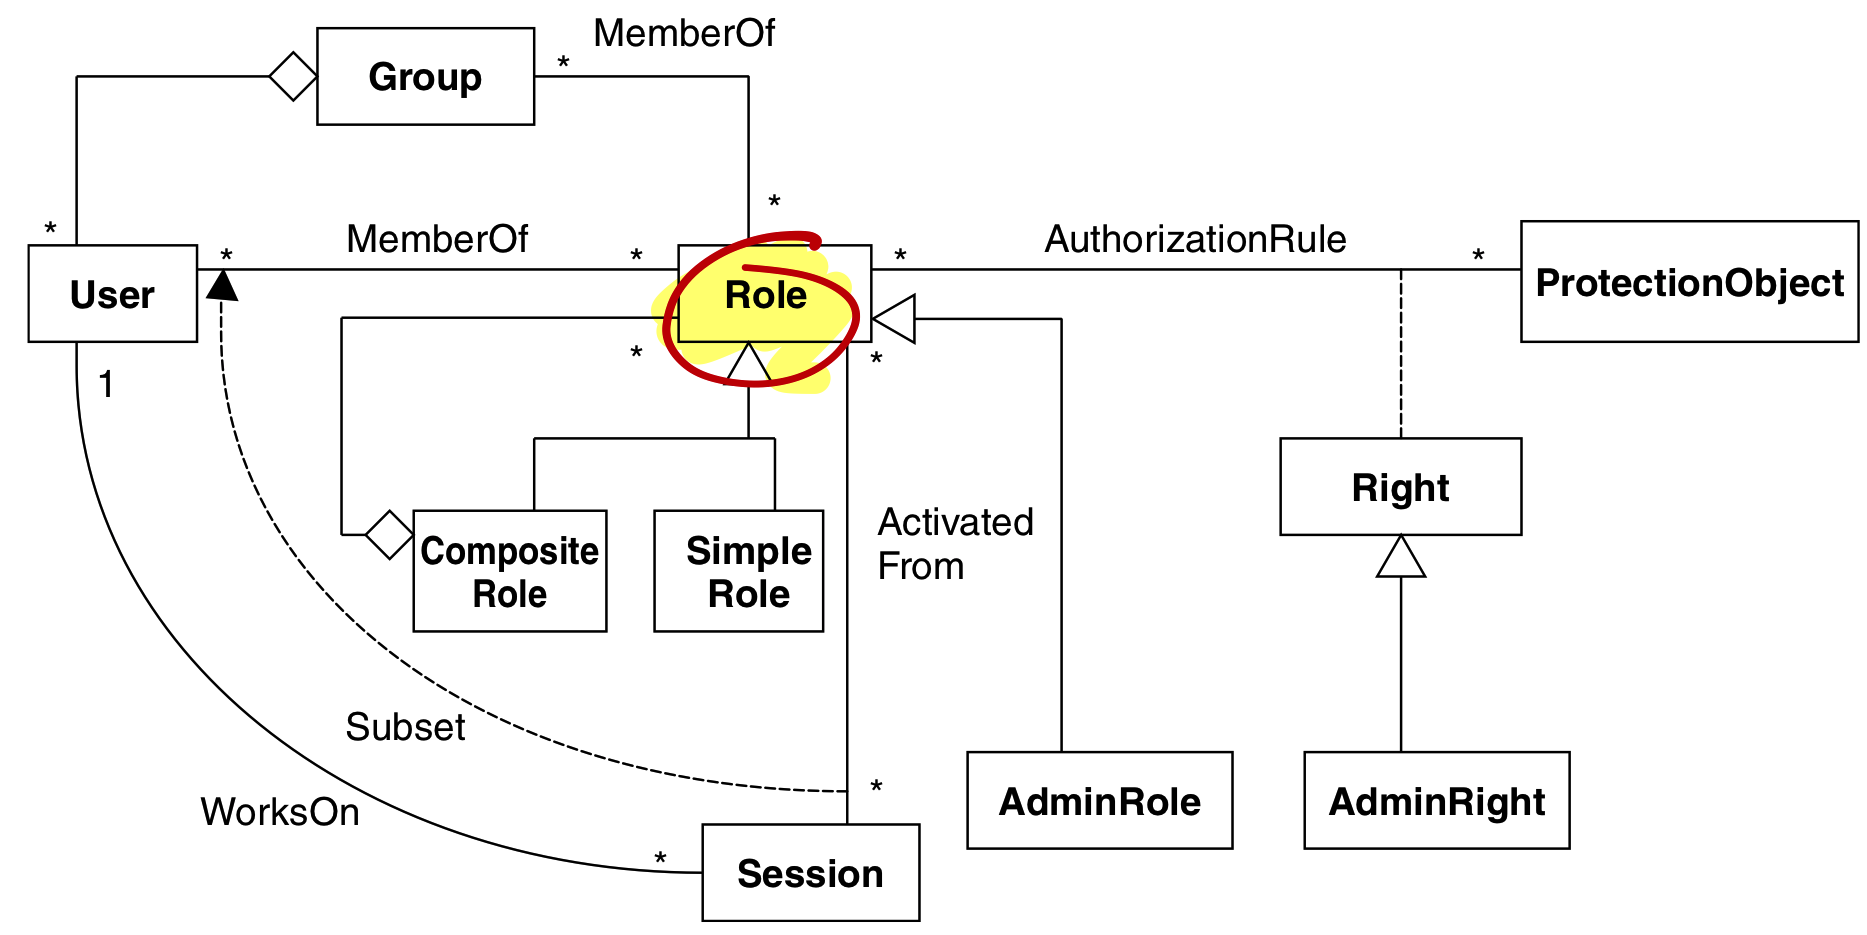
\includegraphics[width=\textwidth]{chapter/01basic/rolebasedaccesscontroladvanced.png}

\subsubsection*{Composite Pattern}
Statt einer simplen Assoziation zwischen User und Role könnte auch mit dem Composite-Pattern gearbeitet werden, um diese Abhängigkeit zu modellieren.

\subsubsection*{Administration}
Wie ebenfalls bereits im Authorization-Pattern erwähnt kann auch dieses Modell zielgerichtet um Administrations-Elemente erweitert werden.
Auf diese Weise kann zusätzliche Klarheit im System geschaffen werden, wer genau für was zuständig ist.

\subsubsection*{Abstract Session}
Um die Möglichkeiten auf die Spitze zu treiben, sei hier auch das Abstract Session Pattern erwähnt: Die Abhängigkeit einer Session kann so direkt ins Security Modell ''miteinmodelliert'' werden.

\subsection*{Vor- \& Nachteile}
\begin{itemize}
	\item Die Zusammenfassung zu Gruppen ermöglicht eine vereinfachte Administration der gesamthaft vorhandenen Berechtigungen
	\item Veränderungen in der realen Organistaionstruktur (Neuzugänge, Abgänge, Jobwechsel etc.) können einfacher auf das Sicherheitskonzept abgebildet werden
	\item Ein Subjekt kann durch mehrere Sessions verschiedene Funktionen auf einmal wahrnehmen
	\item Theoretisch können Gruppen wiederum in Gruppen zusammengefasst werden (Yay, even more complexity...)
	\item Konzeptionelle Komplexität nimmt durch die neuen Elemente wiederum zu!
\end{itemize}

\subsection*{Beispielanwendungen}
\begin{itemize}
	\item 
\end{itemize}

%\chapter*{Examples}

\section*{Glossary Example}

\gls{sqlite} ist ein Glossar Eintrag. Lorem ipsum dolor sit amet, consetetur sadipscing elitr, sed diam nonumy eirmod tempor invidunt ut labore et dolore magna aliquyam erat, sed diam voluptua. At vero eos et accusam et justo duo dolores et ea rebum.

\section*{Bibliography and Citation Example}

Dies ist ein Zitat aus einem Buch\cite{Matthews201111}. Lorem ipsum dolor sit amet, consetetur sadipscing elitr, sed diam nonumy eirmod tempor invidunt ut labore et dolore magna aliquyam erat, sed diam voluptua. At vero eos et accusam et justo duo dolores et ea rebum.

Lorem ipsum dolor sit amet, consetetur sadipscing elitr, sed diam nonumy eirmod tempor invidunt ut labore et dolore magna aliquyam erat, sed diam voluptua. At vero eos et accusam et justo duo dolores et ea rebum. Stet clita kasd gubergren, no sea takimata sanctus est Lorem ipsum dolor sit amet. Lorem ipsum dolor sit amet, consetetur sadipscing elitr, sed diam nonumy eirmod tempor invidunt ut labore et dolore magna aliquyam erat, sed diam voluptua. At vero eos et accusam et.

\section*{Table Example}
\subsection*{All Columns same Width}
\begin{tabularx}{\textwidth}{X X X X} \beforeheading
\heading{Heading 1} & \heading{Heading 2} & \heading{Heading 3} & \heading{Heading 4} \\\afterheading
Cell 1,1 & Cell 1,2 & Cell 1,3 & Cell 1,4 \\\normalline
Cell 2,1 & Cell 2,2 & Cell 2,3 asdf kahsdfkahsklf haskhfkasdhf kjasdhfkjas hfkajsh fkjasdhf kjasdhf kashdfk jhasdkfh askjdhf askh f & Cell 2,4 \\\normalline
Cell 3,1 & Cell 3,2 & Cell 3,3 & Cell 3,4 \\\lastline
\end{tabularx}

\subsection*{Column Alignment \& Filler}
\begin{tabularx}{\textwidth}{l c r X} \beforeheading
\heading{Left Aligned} & \heading{Centered} & \heading{Right Aligned} & \heading{Filler} \\\afterheading
Cell 1,1 & Cell 1,2 & Cell 1,3 & Cell 1,4 asdf kahsdfkahsklf haskhfkasdhf kjasdhfkjas hfkajsh fkjasdhf kjasdhf kashdfk jhasdkfh askjdhf askh f \\\normalline
Cell 2,1 & Cell 2,2 & Cell 2,3 & Cell 2,4 asdf kahsdfkahsklf haskhfkasdhf kjasdhfkjas hfkajsh fkjasdhf kjasdhf kashdfk jhasdkfh askjdhf askh f \\\normalline
Cell 3,1 & Cell 3,2 & Cell 3,3 & Cell 3,4 asdf kahsdfkahsklf haskhfkasdhf kjasdhfkjas hfkajsh fkjasdhf kjasdhf kashdfk jhasdkfh askjdhf askh f \\\lastline
\end{tabularx}
%\chapter{Einleitung}

\section{Aufgabenstellung}


\section{Involvierte Personen}
\subsection{Team}
\subsubsection*{Manuel Alabor}
Lorem Ipsum

\subsubsection*{Alexandre Joly}
Lorem Ipsum

\subsubsection*{Michael Weibel}
Lorem Ipsum


\subsection{Betreuung \& Bewertung}
\subsubsection*{Prof. Hans Rudin}
Lorem Ipsum

\subsubsection*{Kevin Gaunt}
Lorem Ipsum

\subsubsection*{Daniel Hiltebrand}
Lorem Ipsum
%\chapter{Projektmanagement}

\section{Plattformen}
\subsection{Thesis}
Die Bachelor-Thesis ist zwecks vereinfachter Zusammenarbeit im LaTeX-Format in folgendem Git-Repository abgelegt:
\begin{itemize}
	\item \url{https://github.com/mweibel/BA-Dokumentation}
\end{itemize}

\subsection{Planung, Tracking \& Zeitrapportierung}
Zur Planung und Verfolgung des aktuellen Arbeitsfortschrittes sowie zur Zeitrapportierung wird eine Redmine-Installation verwendet:
\begin{itemize}
	\item http://redmine.alabor.me/projects/ba2013
\end{itemize}

\subsection{Code Repository}
Zur Versionierung von Quellcode sowie zentraler Verwaltung dessen wird ein Git-Repository auf github.com verwendet:
\begin{itemize}
	\item \url{https://github.com/mweibel/ba}
\end{itemize}

\subsection{Andere Artefakte}
Jegliche andere Artefakte werden zentral auf einem Dropbox-Share versioniert und verwaltet.


\section{Meetings}
\subsection{Wöchentliches Statusmeeting}
Es findet jeweils am Mittwoch um 10 Uhr ein woöchentliches Statusmeeting statt. Die Sitzung wird abwechslungsweise jeweils von einer Person aus dem Projektteam geführt und von einer anderen protokolliert.

\subsection{Protokollierung}
Alle Protokolle zu abgehaltenen Meetings sind im Thesis-Git-Repository einsehbar:
\begin{itemize}
	\item \url{https://github.com/mweibel/BA-Dokumentation}
\end{itemize}

\section{Phasenplanung}
TODO

\section{Meilensteine}
TODO

\section{Personelles}
\subsection{Abwesenheiten}
\begin{tabularx}{\textwidth}{l l l X} \beforeheading
\heading{Wer?} & \heading{Von} & \heading{Bis} & \heading{Grund} \\\afterheading
MAL & 02.04.2013 & 05.04.2013 & Militär \\\normalline
MAL & 23.05.2013 & 31.05.2013 & Militär (Mitarbeit in der zweiten Hälfte machbar) \\\lastline
\end{tabularx}
% \input{chapter/04mychapter}
% ...


% List of figures & glossary
%%%%%%%%%%%%%%%%%%%%%%%%%%%%
\listoffigures
\printglossary[style=altlist,title=Glossar]

% Bibliography
%%%%%%%%%%%%%%
\bibliographystyle {alpha}
\bibliography{index/bibliography}


% Attached sources
%%%%%%%%%%%%%%%%%%
%\chapter{Anhang}

\input{attachments/meetings}
\newpage
\input{attachments/aufgabenstellung}


\end{document}